\newcommand{\srroot}{Chapters/sr}

%%%%%%%%% TITLE
\section{Multi-frame face super-resolution}


\begin{abstract}

Face verification and recognition problems have seen rapid progress in recent years, however recognition from small size images remains a challenging task that is inherently intertwined with the task of face super-resolution. Tackling this problem using multiple frames is an attractive idea, yet requires solving the alignment problem that is also challenging for low-resolution faces. Here we present a holistic system for multi-frame recognition, alignment, and superresolution of faces. Our neural network architecture restores the central frame of each input sequence additionally taking into account a number of adjacent frames and making use of sub-pixel movements. We present our results using the popular dataset for video face recognition (YouTube Faces). We show a notable improvement of identification score compared to several baselines including the one based on single-image super-resolution.


\end{abstract}

\subsection{Introduction} Face recognition systems have seen a great progress over the last several years with super-human recognition accuracy attainable in many scenarios. However, the accuracy of recognition degrades very significantly when dealing with very low resolution faces. In such conditions, the tasks of recognition and increasing the effective resolution (\textit{super-resolution}) become intertwined and necessitate joint solution. Indeed, developing  super-resolution techniques without regard for recognition often leads to face \textit{hallucination}, i.e.\ a process that creates plausibly looking faces lacking personal specifics. On the other hand, super-resolution has been known to benefit from recognition for a long time \cite{baker2002limits}.

\begin{figure}[t]
%\begin{wrapfigure}{i}{0.5\textwidth}
\includegraphics[width=\columnwidth]{\srroot/images/ytube/teaser.png}
\caption{Results of different super-resolution convolutional networks on samples from the Youtube Faces (YTF) dataset. From left to right: ground truth, bicubic upsampling,  single-frame superresolution, super-resolution from 25 frames without alignment (ours), super-resolution from 25 frames with warping subnetwork (ours).}
\label{fig:teaser}
%\vspace{10pt}
\end{figure}



While single-image super-resolution has recently drawn considerable attention \cite{ZhuLLT16, TuzelTH16}, super-resolution over large magnification factors can benefit significantly from information accumulated over multiple images, e.g.\ using adjacent frames in a surveillance stream or a video. Traditionally, multi-frame super-resolution has required rigid or non-rigid alignment with sub-pixel accuracy \cite{capel2003computer}. 
At the same time, faces have complex and deformable shapes leading to complex two-dimensional motion patterns which makes motion estimation hard to accomplish at sub-pixel precision. Generally, such precise alignment cannot be accomplished using low-level cues alone, and therefore requires high-level understanding/recognition of face geometry.



Motivated by all these observations, we present a system that performs multi-frame super-resolution by tackling all three inter-related problems, namely super-resolution, non-rigid alignment, and recognition, jointly and simultaneously. The tasks are implemented as modules of a deep neural network architecture that is trained in an end-to-end fashion on a dataset of realistic face videos \cite{WolfHM11}. The forward pass in our network involves pairwise alignment of pairs of frames performed in parallel with feature extraction, while the super-resolution is accomplished by a subsequent reconstruction module that takes warped features of the multiple frames into account. The learning process is driven by a combination of loss functions that includes the recognition-related loss ensuring that the super-resolution process reconstructs person-specific traits. 




%Here, we propose and evaluate a deep system that embraces all the aforementioned features: super-resolution, caring for recognition, multiple frames usage, motion recovering and avoiding hallucination. The system is trained end-to-end. \emph{Face Warping} sub-network is responsible for predicting the motion compensation transformation to align pairs of frames in a video-sequence to match one reference frame. The predicted transforms are applied to deep features of the frames in the input sequence, computed with \emph{Frame Feature extractors}. \emph{Combining} sub-network accepts all the transformed frames features and reconstructs the central frame in the sequence. 
Overall, while individual components of our system have been proposed in previous works, to the best of our knowledge, our work is the first that builds a systems that combines face super-resolution, recognition and alignment in a holistic manner. 
We evaluate the proposed architecture on the hold-out part of the YouTube Faces (YTF) dataset (\cite{WolfHM11}). We demonstrate good face verification  performance for the restored images using standard protocols adopted for the YTF dataset. We also show benefits of using multiple frames along with \emph{Face Warping} sub-network over the single-image approach. 
 We additionally compare our approach with  state-of-the-art face hallucination method \cite{ZhuLLT16} and find our method to perform better on the YouTube Faces dataset.

In the remainder of this work, we review the most related approaches in \ref{sec:related} describe the components of the proposed system in \ref{sec:video} and \ref{sec:loss} demonstrate the super-resolution results in \ref{sec:exps} and conclude with a short summary in \ref{sec:summary}. 

\subsection{Related work}
\label{sec:related}

\subsection{Face super-resolution approaches}

Initially, super-resolution problem has been formulated for low-resolution image sequence that can be used to produced one image of higher resolution. Under this approach, reconstruction constraints are used to make sure that resulting high-resolution image is consistent with the input sequence. 
Maximum a posteriori (MAP) framework has been used in \cite{HardieBA97, SchultzS96, baker2002limits} to take into account such reconstruction constraints along with priors on the high-resolution image.

Precise image registration has been shown to be very important for multi-image \cite{HardieBA97, IraniP91, SchultzS96} and super-resolution methods but is rarely achievable for real  low-resolution data, especially for images depicting non-rigid objects such as faces. In the case of multi-image super-resolution, approximate low-parametric registration could be used instead. For single-image super-resolution, such registration with canonical pose can also be used in order to use stronger face-specific priors \cite{LiuSF07}.


Having assumed ideal image registration, Baker \emph{et al.} \cite{baker2002limits} demonstrate the effect of introducing additional recognition-based prior. The authors include it into the task formulation as additional constraints based on particular examples from  training set chosen by similarity to the regions of the input image.  Later, more advanced techniques for modeling such face-specific constraints were introduced in \cite{LiuSF07} for single-image face super-resolution. The authors decomposed such constraints to \emph{global} and \emph{local} constraints. A similar idea was also adopted in \cite{TuzelTH16} to build a ConvNet architecture for single-image face super-resolution.


%TODO : maybe elaborate on this.
%correspondence between low res and high-res patches 
%dictionary learning: faces \cite{YangWLCH12, TianT16}, direct patch correspondence :  \cite{MaZQ10}, methods are also very dependent on alignment, general and CNN :  \cite{DongLHT16} 

\subsection{Deep learning for face super-resolution}

Several recent deep learning approached \cite{TuzelTH16,ZhuLLT16,xu2017learning,huang2017wavelet} focus on single-image face super-resolution problem.
Tuzel \emph{et al.} \cite{TuzelTH16} suggested the end-to-end learning scheme to obtain high quality results even in the case of 8x down-sampling. The architecture includes two parts corresponding to global and local modeling of the face features. In the \emph{global} network, the fully-connected layers are used to capture the global face structure, while the \emph{local} part consists of convolution layers that are used to model local face features. Additionally, authors apply adversarial learning to achieve more realistic results. 
Below, we use the \textit{Perceptual loss} for the similar goal.

Xu \emph{et al.} \cite{xu2017learning} also use generative adversarial networks (GANs) \cite{goodfellow2014generative} for single-image face super-resolution. The authors introduce additional recognition-based losses. First, feature matching loss ensures that reconstructed high-resolution image and ground truth image have similar features extracted from the discriminator network. This approach resembles \textit{Perceptual losses}.  Second, multi-class discriminator was used to learn one generator network for two different domains of texts and faces. %The authors demonstrate visual improvement of combination of feature-level and GAN losses over using only GAN loss. Together these losses help to build a strong prior on generated images and achieve better qualitative and quantitative results. 


Zhu \emph{et al.}~\cite{ZhuLLT16}  proposed a cascaded scheme that includes iterative high-resolution image refinement and pose estimation from these refined images. This approach is motivated by the fact that face super-resolution and face pose estimation tasks are related, and it is easier to increase image resolution knowing the pose of the face and vice versa. Special gated architecture is introduced to effectively combine high-frequency and low-frequency information and make use of face pose estimated at previous scale levels.

Huang \emph{et al.} \cite{huang2017wavelet} use another recognition-based loss: the proposed neural network is trained to predict wavelet transform coefficients which helps to capture and match information at different scales.

All the aforementioned methods only consider single-frame face super-resolution/restoration. To the best of our knowledge, none of the recent works on deep face super-resolution consider multi-frame scenario. It should also be mentioned that methods \cite{TuzelTH16,xu2017learning,huang2017wavelet} use pre-aligned images for training and testing. (However, \cite{huang2017wavelet} demonstrate very impressive results for difficult face poses.) In contrast, we stick to 'more real' scenario when no alignment is applied to high-resolution ground-truth images before down-sample them. 


\subsection{Restoration and recognition}
%\cite{Hennings-YeomansBK08, ZhangYZNH11}
%The idea of combining the two tasks of face image restoration and face recognition has been investigated in several works


Initially, recognition was incorporated into face super-resolution in the form of face-specific priors \cite{baker2002limits, LiuSF07}. Several works considered an explicit combination of face recognition and face restoration tasks: \cite{Hennings-YeomansBK08, ZhangYZNH11}.
The proposed approaches perform recognition using a limited number of gallery images. In parallel, they reconstruct the input image and classify it based on labels of the most relevant examples found in the train set. Here we work in a different setting using a feed-forward deep neural network to produce the restored high-resolution image without using the gallery set at test time.

\subsection{Deep learning for video-based super-resolution}
As mentioned earlier, video data bring more useful information compared to isolated frames and can be used to enhance the restoration algorithms. Naturally, most recent deep learning approaches, which focus on video super-resolution \cite{LiaoTLMJ15, SongDQ16, TaoGLWJ17}, use motion estimation to align a number of subsequent frames to make use of sub-pixel motion and reveal more object details. Liao~\emph{et al.}~\cite{LiaoTLMJ15} use different optical flow methods to generate super-resolution "drafts". Such drafts can then be further combined into the final reconstruction using a number of convolutional layers. Kappeler~\emph{et al.}~\cite{KappelerYDK16} also experiment with different variants of video-based super-resolution architecture incorporating neighbouring frames alignment. 

%here it is interesting to check if Warping Subnet even changes during training => it would be possible to say that we benefit from end-to-end learring in this case.
Our idea is to adopt similar approach based on video-data and frame alignment for human faces. Importantly, we aim not only at enhancing image quality but also at preserving face identities and therefore improving face verification quality for the restored images.
 
   





%\begin{figure*}
%\begin{center}

%\includegraphics[width=\textwidth]{images/method/vgg_loss.pdf}

%\caption{General scheme of learning super-resolution with perceptual loss. Along with L2 loss, the \textit{Perceptual loss} \cite{JohnsonAF16} is used, that is the loss computed for high-level features extracted from pre-trained CNN. The weights of the pre-trained CNN are fixed during training. See \ref{sec:vgg_loss} for the details.}

%\label{fig:vgg_loss}

%\end{center}

%\end{figure*}



\section{Evaluated approaches}
\label{sect:method}
\bigskip
\indent\textbf{Face recognition for the low-quality image domain}\\
%\subsubsection{Face recognition for the low-quality image domain}
\label{sect:strategies}
In this work we consider and compare two main approaches to face recognition for surveillance data: 1) restoration-based approach and 2) domain adaptation of existing face recognition neural networks. 

We consider two facial image domains: \begin{itemize}
\item domain $T: \{X^{T}_{i} \}_{i=0}^{N_T}$ that includes low-quality facial images $X^{T}_{i}$ captured using surveillance cameras. Usually, there are no identity labels provided, as assigning identity labels is quite challenging and may not even be feasible.
\item domain $S: \{(X^{S}_{i}, Y^{S}_{i})\}_{i=0}^{N_S}$ that includes facial images $X^{S}_{i}$ harvested from the Internet. These images are usually of higher quality and are taken in good lighting conditions. We assume that the data in this domain are supplied with identity labels $Y_i$.
\end{itemize}  

According to the available labeling, we can consider two different pipelines for building face recognition systems for surveillance data. The first option is the restoration-based approach when we use transform $F^{T \rightarrow S}: T \longrightarrow S$ as a face restoration method and then apply existing recognition neural network $R^{S}$ that is pre-trained on images from the domain $S$. The second option is to use the transform $F^{S \rightarrow T}: S \longrightarrow T$ to transfer the large collections of labeled training data to the target domain of surveillance images. In this scenario, we retrain the existing face recognition networks resulting in the new adapted model $R^{T}$.

More formally, we consider the following two pipelines for face recognition in the domain $T$.  We denote $d^{T}$ and $d^{S}$ the descriptors produced by the domain-specific face recognition models $R^{T}$ and $R^{S}$. These descriptors may be used e.g.\ to identify matching and non-matching faces based on the distances between them. 
 
$F^{T \rightarrow S}: T \longrightarrow S$ and $F^{S \rightarrow T}: B \longrightarrow A$ are the image-level domain transfer mappings. In the restoration-based approach, we train the recognition model $R^{S}$ using labeled data  $\{(X^{S}_{i}, Y^{S}_{i})\}$ where $X^{S}_{i} \subseteq B$. We then test the learned model by computing the descriptors $d^{S}$ after applying the network $F^{T \rightarrow S}$:  $d^{S} = R^{S}(X^{T\rightarrow S}) = R^{S}(F^{T \rightarrow S}(X^{T}))$

In the domain adaptation approach, we train the recognition network $R^{T}$ using labeled data $\{(X^{S \rightarrow T}_{i}, Y^{S}_{i})\}$, where the training examples $X^{S \rightarrow T }_{i} = F^{S \rightarrow T}(X^{S}_i)$, $X^{S}_i \subseteq S$ are obtained by transforming the high-quality images to the low-quality domain using the learned transformation $F^{S \rightarrow T}$. In this case, we apply the learned network directly to the low-quality images by computing and working with their descriptors $d^{T} = R^{T}(X^{T})$. The two approaches are compared below.


%image describing train and test time for both schemes
\bigskip
\indent\textbf{Learning domain transfer mappings}\\
%\subsubsection{Learning domain transfer mappings}
\label{sect:domain_transfer}
We use the CycleGAN approach~\citep{ZhuPIE17} to simultaneously learn the domain transfer mappings in both directions: $ F^{T \rightarrow S}: T  \longrightarrow S$ (restoration-based approach) and  $F^{S \rightarrow T}: S \longrightarrow T$ (domain adaptation approach). Here we describe the objective functions used for learning the domain transfer architecture.

We use the variant of CycleGAN similar to the one introduced in \citep{LiuNIPS2017} as we found it resulting in more stable and visually more plausible results for our task than the original framework \citep{ZhuPIE17}. Following \citep{LiuNIPS2017}, we decompose the domain transfer mappings into the compositions of encoders and generators: $F^{T \rightarrow S} = G^{S} \odot E^{T} $ and $F^{S \rightarrow T} = G^{T} \odot E^{S} $. Here, the encoders $E^{T}$ and $E^{S}$ transfer input images to the latent space, and generators $G^{S}$ and $G^{T}$ map the input latent codes to the domains $S$ and $T$.
 
For inputs $X^{T} \subseteq T $ and $X^{S} \subseteq S $ the results of their transfer to the opposite domain will be:
\begin{equation}
    X^{T \rightarrow S} = F^{T \rightarrow S}(X^{T}; \theta^{T}_F) = G^{S}(E^{T}(X^{T}))  
\end{equation}
\begin{equation}
    X^{S \rightarrow T} = F^{S \rightarrow T}(X^{S}; \theta^{S}_F) = G^{T}(E^{S}(X^{S}))
\end{equation}

The objective function used by the CycleGAN approach for learning is composed of the two symmetric parts:
\begin{equation}
\mathcal{L} = \mathcal{L}^{T} + \mathcal{L}^{S},
\end{equation} where $\mathcal{L}^{T}$ further decomposes as:
\begin{equation}\label{eq:domain_loss}
     \mathcal{L}^{T} = \mathcal{L}_{\text{GAN}}^T + \lambda_1 \mathcal{L}_{\text{cycle}}^T + \lambda_2 \mathcal{L}_{\text{rec}}^T,
\end{equation}
while $\mathcal{L}^{S}$ has same structure as $\mathcal{L}^{T}$:
\begin{equation}\label{eq:domain_loss2}
     \mathcal{L}^{S} = \mathcal{L}_{\text{GAN}}^S + \lambda_1 \mathcal{L}_{\text{cycle}}^S + \lambda_2 \mathcal{L}_{\text{rec}}^S,
\end{equation}


We now describe each of the terms in \eq{domain_loss}.
The GAN loss serves as the optimization objective for the domain transfer: 

\begin{dmath}
\mathcal{L}_{\text{GAN}}^A = 
    \min_{\theta^{S}_F} \max_{\theta^{T}_D} \mathbb{E}_{x \sim p_{X^{T}}} \log D^{T}(x) +
    \mathbb{E}_{x \sim p_{X^{S}}} \log \big(1 - D^{T}(F^{S \rightarrow T}(x)) \big)\,
\end{dmath}


Here, $D^{T}(X;\theta^{T}_D)$ and $D^{S}(X;\theta^{S}_D)$ are discriminators for the domains $T$ and $S$ that are trained in parallel with the training of the domain transforms.

The other two terms are the so-called cycle consistency loss: 
\begin{equation}
\mathcal{L}_{\text{cycle}}^T = L_1(F^{S \rightarrow T}(F^{T \rightarrow S}(X^{T})), X^{T})  
\end{equation}
and the reconstruction loss:
\begin{equation}
\mathcal{L}_{\text{rec}}^T = L_1(G^{T}(E^{T}(X^{T})), X^{T}) 
\end{equation}
In both terms, $L_1(\cdot,\cdot)$ denotes the $L_1$ distance.

We show the results of transferring the Internet and surveillance images to the other domain in figure \ref{fig:lr_hr_gan_res_ytube_initial_degraded}. While these results look interesting, we do not analyze their visual quality, as we are ultimately interested in the recognition performance rather than obtained visually-convincing images.

\bigskip
\indent\textbf{Learning face recognition models}\\
%\subsubsection{Learning face recognition models}
\label{sect:face_recognition}
In both scenarios that we compare in this paper, we need to train a face recognition model that turns images into vectorial descriptors. This happens either in domain $S$ (in the face restoration approach) or in domain $T$ (in the domain adaptation approach).

In either case, the goal of the training is to build a deep convolutional network that converts face images to the descriptors, such that matching face images have close descriptors and non-matching face descriptors have dissimilar descriptors. We use the Binomial Deviance loss~\citep{Yi14} to perform such training \eq{bindev}. We note that the choice of a particular metric learning loss is orthogonal to our study.

Alternatively to the models trained using the setting discussed above, we also consider reusing the VGG face model trained by the authors of~\citep{parkhi2015deep} on the VGG-face dataset.
\section{Experiments}
\label{sect:experiments}

We now perform evaluation and the comparison of the two approaches and their variants. 


\bigskip\indent\textbf{Datasets and protocols} 
%\subsubsection{Datasets and protocols}

\label{sect:datasets}

\bigskip\indent\textbf{Surveillance data}\\
%\subsubsubsection{Surveillance data}
\label{sect:surveillance}
For the surveillance image domain ($T$, as denoted in \sect{strategies}), we have obtained a surveillance dataset comprising faces from five cameras in Moscow subway. Our dataset consists of two subsets of images, denoted as \texttt{LR} (low-resolution) and \texttt{HR} (high-resolution) according to their size in pixels. Sizes are calculated as the face bounding box heights. Mean face heights for \texttt{LR} and \texttt{HR} subsets were $49.72$ and $106.19$ pixels correspondingly. The \texttt{LR} images range from $37$ to $63$ pixels, and \texttt{HR} images from $75$ to $224$. The DLib \cite{dlib09} library was used for face detection and subsequent alignment. 
 
Generally, the identities of people occurring in the video are unknown, and therefore we mine matching faces in the dataset by considering temporal tracks in videos. We assume that face images from different tracks are non-matching. The matching pairs then correspond to pairs of faces from the same track, such that one image belongs to the LR subset and the other belongs to the HR subset. Columns 1 and 3 in \fig{lr_hr_gan_res_ytube_initial_degraded} show some examples of matched pairs. Usually, the quality of face images increases when the person approaches the camera, and therefore \texttt{HR}-subset images are often (but not always) visually better than those present in the \texttt{LR} subset. The division into \texttt{LR} and \texttt{HR} subsets is introduced to ensure that the matched pairs of frames correspond to distinct frames of the temporal tracks. We stress that the mined matching pairs are used for evaluation (testing) only and are not used for training of any networks in our experiments.

We use $100$ identities that are present in both \texttt{LR} and \texttt{HR} for parameter validation and $100$ identities for test. For each of the test identity, there is a pair of matching tracks (one LR track and one HR track). The goal of algorithms is then to build descriptors that would be similar for frames coming from the HR and the LR tracks of the same identity, and would be dissimilar for the HR and the LR tracks corresponding to different identities.

$7,535$ images of identities not present in the test set are used for training the unsupervised domain transfer described in \sect{domain_transfer} (tracking-based information was not used to train the ConvNets). The mean number of frames for each identity in \texttt{LR} and \texttt{HR} test data are $18.62$ and $17.72$ correspondingly.
 
 To evaluate the recognition quality, we match identities across the \texttt{LR} and \texttt{HR} in the following way: we calculate the cosine similarity between the frame set $t_{id_1}^{LR}$ of identity $id_1$ and the frame set, $t_{id_2}^{HR}$ of identity $id_2$ by averaging the similarities of each pair of frames: 

 \begin{align}
     S(t_{id_1}^{LR},t_{id_2}^{HR}) = \sum_{i=0, j= 0}^{|t_{id_1}^{LR}|, |t_{id_2}^{HR}|} S(f_{id_1,i}^{LR},f_{id_2,j}^{LR} ), \\
     S(f_{id_1,i}^{LR},f_{id_2,j}^{LR} ) =  cos(d_{id_1,i}^{LR},d_{id_2,j}^{LR}),
 \end{align}
 where $d_{id_1,i}^{LR}$,$d_{id_2,j}^{HR}$ are the descriptors of the corresponding frames calculated by face recognition neural network $R$ \ref{sect:face_recognition}.
%f_{id_1,i}^{low} \subseteq t_{id_1}^{low} , %f_{id_2,j}^{low} \subseteq t_{id_1}^{low}

%\subsubsection{Evaluation metrics}
\bigskip\indent\textbf{Evaluation metrics}\\
We focus our evaluation on the surveillance data domain. As already mentioned above, during evaluation, we compare pairs of \textit{tracks}, where the first track comes from the \texttt{LR} subset and the second track comes from the \texttt{HR} subset. 

When comparing the two tracks using the recognition metrics, we match all possible pairs of frames and compute the mean average cosine similarity between the computed descriptors over all pairs (more sophisticated schemes involving minimal pairs did not result in better performance). Depending on whether the mean average cosine similarity is higher or lower than a certain threshold $\tau$, we treat a certain pair of tracks as matching or non-matching.

 By considering various $\tau$, we then compute the \textit{ROC curve}, the area under the ROC curve (ROC AUC), the $100$\% - EER (Equal Error Rate) statistics, and the average precision (AP) metrics. 


\bigskip\indent\textbf{Internet data}\\
%\subsubsubsection{Internet data}
For the Internet image domain ($S$, as denoted in \sect{strategies}) we use two face recognition datasets: YouTube Faces (YTF) \cite{WolfHM11} and the VGG Face datasets \cite{parkhi2015deep}. %Celeb-A \cite{liu2015faceattributes},

%todo check
%The Celeb-A dataset~\cite{liu2015faceattributes} consists of $202,599$ images of high quality and is used for training CycleGAN-based  domain transfer described in \sect{domain_transfer}. 


% ----------------to main intro
 The Youtube Faces (YTF) dataset~\cite{WolfHM11} and the VGG Face dataset~\citep{parkhi2015deep} are used for the finetuning of the face recognition neural network as described in \sect{face_recognition}.

%YTF consists of $3,425$ videos of $1,595$
% people collected from YouTube, with an average of 2 videos per identity. The VGG Face dataset contains $2,6$M images of $2,622$ identities. 

We show that face recognition improves, when using our CycleGAN-based data augmentation when trained on either YTF or VGG Face. Generally, YTF and VGG Face represent two different types of face images that can be mined from the Internet (with YTF having lower quality).





%All the images in the four mentioned datasets are aligned in the same way: DLib is used for feature detection and alignment by $3$ eyes and nose feature-points, so that their target positions are the following :


\bigskip\indent\textbf{Compared variants of recognition networks} \\
%\subsubsection{Compared variants of recognition networks}
\label{sect:ft}
We compare the following adaptation/transfer strategies for training the recognition networks:
\begin{itemize}

\item \textit{no ft} -- the pre-trained VGG-face model~\cite{parkhi2015deep} with no re-training is used to compute descriptors of the surveillance-domain images.


\item \textit{ft initial} -- the VGG-face model is fine-tuned using the original version of the YTF or the VGG Face datasets (no domain adaptation). 

\item \textit{ft degraded} -- the VGG-face model fine-tuned using the degraded version of the YTF or VGG Face datasets transferred to the target (surveillance) domain (using domain adaptation),

\item \textit{ft union} -- the VGG-face model fine-tuned using \textbf{both} the initial and the degraded versions  of the YTF or VGG Face datasets (using domain adaptation). 

\end{itemize}

The YTF dataset images and the corresponding degraded images are shown  in \fig{lr_hr_gan_res_ytube_initial_degraded} (the two last columns).
%The two last variants \textit{ft degraded} and \textit{ft union} perform domain adaptation, as all or part of the training data are transferred to the target domain.



\bigskip\indent\textbf{Training details}  \\
%\subsubsection{Training details}
\label{sect:training}
The CycleGAN-based domain transfer consists of $3$ types of modules (see \sect{domain_transfer}).
Encoders $E_T$ and $E_S$ have the following architecture:
\begin{center}
\begin{scriptsize}
\begin{tabular}{l | c c c c c c c}
\hline
  \#conv layer      &1   &2      &3    &4     &5    &6    &7     \\
  num of filters    &32  &64     &128  &128   &128  &128  & 128  \\
  kernel size       &3   &3      &3    &3     & 3   &3    &3     \\
  stride/pad        &1/0 &2/1    &2/1  &1/1   &1/1  &1/1  & 1/1  \\
  \#res block       & -  & -     & -   & 0    &0    &1    &1     \\
\hline
\end{tabular}
\end{scriptsize}
\end{center}
\vspace{0.5em}

% EncShared(
%   (from_img): ModuleList(
%     (0): Conv2d(3, 32, kernel_size=(1, 1), stride=(1, 1))
%   )
%   (enc_blocks): ModuleList(
%     (0): Sequential(
%       (0): Conv2d(32, 64, kernel_size=(3, 3), stride=(2, 2), padding=(1, 1), bias=False)
%       (1): InstanceNorm2d(64, eps=1e-05, momentum=0.99, affine=True)
%       (2): LeakyReLU(0.01, inplace)
%     )
%     (1): Sequential(
%       (0): Conv2d(64, 128, kernel_size=(3, 3), stride=(2, 2), padding=(1, 1), bias=False)
%       (1): InstanceNorm2d(128, eps=1e-05, momentum=0.99, affine=True)
%       (2): LeakyReLU(0.01, inplace)
%     )
%   )
% )

% Enc(
%   (enc_blocks): ModuleList(
%   )
%   (res_blocks): ModuleList(
%     (0): ResBlock(
%       (model): Sequential(
%         (0): Conv2d(128, 128, kernel_size=(3, 3), stride=(1, 1), padding=(1, 1), bias=False)
%         (1): InstanceNorm2d(128, eps=1e-05, momentum=0.99, affine=True)
%         (2): LeakyReLU(0.01, inplace)
%         (3): Conv2d(128, 128, kernel_size=(3, 3), stride=(1, 1), padding=(1, 1), bias=False)
%         (4): InstanceNorm2d(128, eps=1e-05, momentum=0.99, affine=True)
%       )
%     )
%     (1): ResBlock(
%       (model): Sequential(
%         (0): Conv2d(128, 128, kernel_size=(3, 3), stride=(1, 1), padding=(1, 1), bias=False)
%         (1): InstanceNorm2d(128, eps=1e-05, momentum=0.99, affine=True)
%         (2): LeakyReLU(0.01, inplace)
%         (3): Conv2d(128, 128, kernel_size=(3, 3), stride=(1, 1), padding=(1, 1), bias=False)
%         (4): InstanceNorm2d(128, eps=1e-05, momentum=0.99, affine=True)
%       )
%     )
%   )
% )

The architecture of generators $G_T$, $G_S$ is as follows:
\begin{center}
\begin{scriptsize}
\begin{tabular}{l | c c c c c c c}
\hline
  \#conv layer      &1      &2    &3     &4    &5    &6    & 7 \\
  num of filters    &128    &128  &128   &128  &64   &32   & 3 \\
  kernel size       &3      &3    &3     & 3   &3    &3    & 1 \\
  stride/pad        &1/1    &1/1  &1/1   &1/1  &1/1  &1/1  & 1/0  \\
  \#res block       &0      &0    &1     &1    &-    &-    & -  \\
\hline
\end{tabular}
\end{scriptsize}
\end{center}
\vspace{0.5em}

Instance normalization~\cite{UlyanovVL17} and Leaky ReLU~\cite{HeZRS15} with negative slope set to $0.01$ are inserted after each of the convolution layers. Except for the last layers of $G_T$ and $G_S$, where \texttt{tanh} non-linearity is used (for the subsequent feeding of the result into the discriminator). To keep the input image size unchanged,  $\times 2$ nearest neighbor upsampling is done before the convolutions $3$ and $4$.
All input images are normalized to $64\times64$ pixels (output images are therefore of the same size). 


% Dec(
%   (to_img): ModuleList(
%     (0): Sequential(
%       (0): Conv2d(32, 3, kernel_size=(1, 1), stride=(1, 1))
%       (1): Tanh()
%     )
%   )
%   (upsample): Upsample(scale_factor=2, mode=nearest)
%   (res_blocks): ModuleList(
%     (0): ResBlock(
%       (model): Sequential(
%         (0): Conv2d(128, 128, kernel_size=(3, 3), stride=(1, 1), padding=(1, 1), bias=False)
%         (1): InstanceNorm2d(128, eps=1e-05, momentum=0.99, affine=True)
%         (2): LeakyReLU(0.01, inplace)
%         (3): Conv2d(128, 128, kernel_size=(3, 3), stride=(1, 1), padding=(1, 1), bias=False)
%         (4): InstanceNorm2d(128, eps=1e-05, momentum=0.99, affine=True)
%       )
%     )
%     (1): ResBlock(
%       (model): Sequential(
%         (0): Conv2d(128, 128, kernel_size=(3, 3), stride=(1, 1), padding=(1, 1), bias=False)
%         (1): InstanceNorm2d(128, eps=1e-05, momentum=0.99, affine=True)
%         (2): LeakyReLU(0.01, inplace)
%         (3): Conv2d(128, 128, kernel_size=(3, 3), stride=(1, 1), padding=(1, 1), bias=False)
%         (4): InstanceNorm2d(128, eps=1e-05, momentum=0.99, affine=True)
%       )
%     )
%   )
%   (dec_blocks): ModuleList(
%     (0): Sequential(
%       (0): Conv2d(128, 64, kernel_size=(3, 3), stride=(1, 1), padding=(1, 1))
%       (1): LeakyReLU(0.01, inplace)
%     )
%     (1): Sequential(
%       (0): Conv2d(64, 32, kernel_size=(3, 3), stride=(1, 1), padding=(1, 1))
%       (1): LeakyReLU(0.01, inplace)
%     )
%   )
% )


%Finally, discriminators $D_A$ and $D_B$ were derived from the
%VGG-face model~\cite{parkhi2015deep}, which was used for calculating face descriptors, leading to the following archiecture:
Finally, discriminators $D_A$ and $D_B$ have the following architecture: 
\begin{center}
\begin{scriptsize}
\begin{tabular}{l |c c c c c }
\hline
  \#conv layer      &1      &2    &3     &4    &5  \\
  num of filters    &64     &128  &256   &256  &1  \\
  kernel size       &3      &3    &3     & 3   &3  \\
  stride/pad        &2/1    &2/1  &2/1   &2/1  &1/0\\
\hline
\end{tabular}
\end{scriptsize}
\end{center}
\vspace{0.5em}
Leaky ReLU \cite{HeZRS15} with negative slope parameter set to $0.01$ is used as an activation. The final fully-connected layer with one output unit is added to $D_A$ and $D_B$.


% Dis(
%   (to_pred): ModuleList(
%     (0): Conv2d(256, 1, kernel_size=(1, 1), stride=(1, 1))
%     (1): Conv2d(256, 1, kernel_size=(1, 1), stride=(1, 1))
%   )
%   (blocks): ModuleList(
%     (0): Sequential(
%       (0): Conv2d(128, 256, kernel_size=(3, 3), stride=(2, 2), padding=(1, 1))
%       (1): LeakyReLU(0.01, inplace)
%     )
%     (1): Sequential(
%       (0): Conv2d(256, 256, kernel_size=(3, 3), stride=(2, 2), padding=(1, 1))
%       (1): LeakyReLU(0.01, inplace)
%     )
%   )
% )


According to the strategies described in \sect{ft}, we fine-tune the VGG-face model, having added new $128$-dimensional embedding layer instead of the initial classification layer (\textit{fc8}). All the results are reported for the \textit{fc7} layer though, as we found it to work better across all compared methods.

ADAM optimization~\cite{Kingma14} was used for both optimization objectives of the domain transfer task and the face recognition task, the learning rates were set to $1e-4$ and $1e-7$ correspondingly. Batch sizes were $16$ and $64$. Learning processes took $50$ epochs for the domain transfer,  and from $80$ to $200$ epochs for the face recognition task. Parameters $\lambda_1$ and $\lambda_2$ were set to $10$ in the loss \eq{domain_loss}. Parameters $\alpha$, $\beta$ and $C$ of the loss \eq{bindev} were set to $2$, $0.5$ and $10$.

For training the face recognition models described in \sect{ft}, the training batches had the following structure: in each batch, there were up to $3$ examples for each class for the VGG Face dataset and up to $10$ examples for the YTF dataset. For the \textit{ft union} model, each training batch was formed out of the examples of one of the domains. The sampling process alternated between the domains at each iteration.


  
 \begin{figure}
  \centering
    \includegraphics[width=\linewidth]{Chapters/face/Fig3.eps}
    \caption{The ROC curves for our face recognition models for different types of test data. Left -- \textit{no ft} model, test data transformation (the curve is denoted by 'restored') improves recognition. Middle -- \textit{ft initial}, the results for test data transformation are not clearly better than the results for initial images. Right -- \textit{ft union} model, the best results are for initial test data, without transformation. See \ref{sect:restoration_comparison} for the details. }\label{fig:roc_oxford_gan_vs_initial}
  \end{figure}

\bigskip\indent\textbf{Does restoration help recognition?} \\
%\subsubsection{Does restoration help recognition?}
\label{sect:restoration_comparison}
We start by assessing the improvement that the restoration process brings to the recognition. For this we evaluate the performance of the three different recognition networks discussed above, when they are applied either to untransformed surveillance-domain images or to surveillance-domain images transformed to the Internet image domain (using the learned mapping $F^{T \rightarrow S}$). See  \fig{lr_hr_gan_res_ytube_initial_degraded} for the example results of the Internet domain  transfer.

The ROC-curves in  \fig{roc_oxford_gan_vs_initial} shows that while the restoration process helps for the \textit{no ft} network, it actually \textit{hurts} for the better-performing \textit{ft initial} and \textit{ft union} networks. While trying to improve the results of the reverse transfer, we have also tried to transfer only the LR subset of the training images, while keeping the HR subset intact, but this lead to uniformly worse results.

We conclude that restoration does not necessarily help the recognition process in our setting. 



\begin{figure}
 \centering
    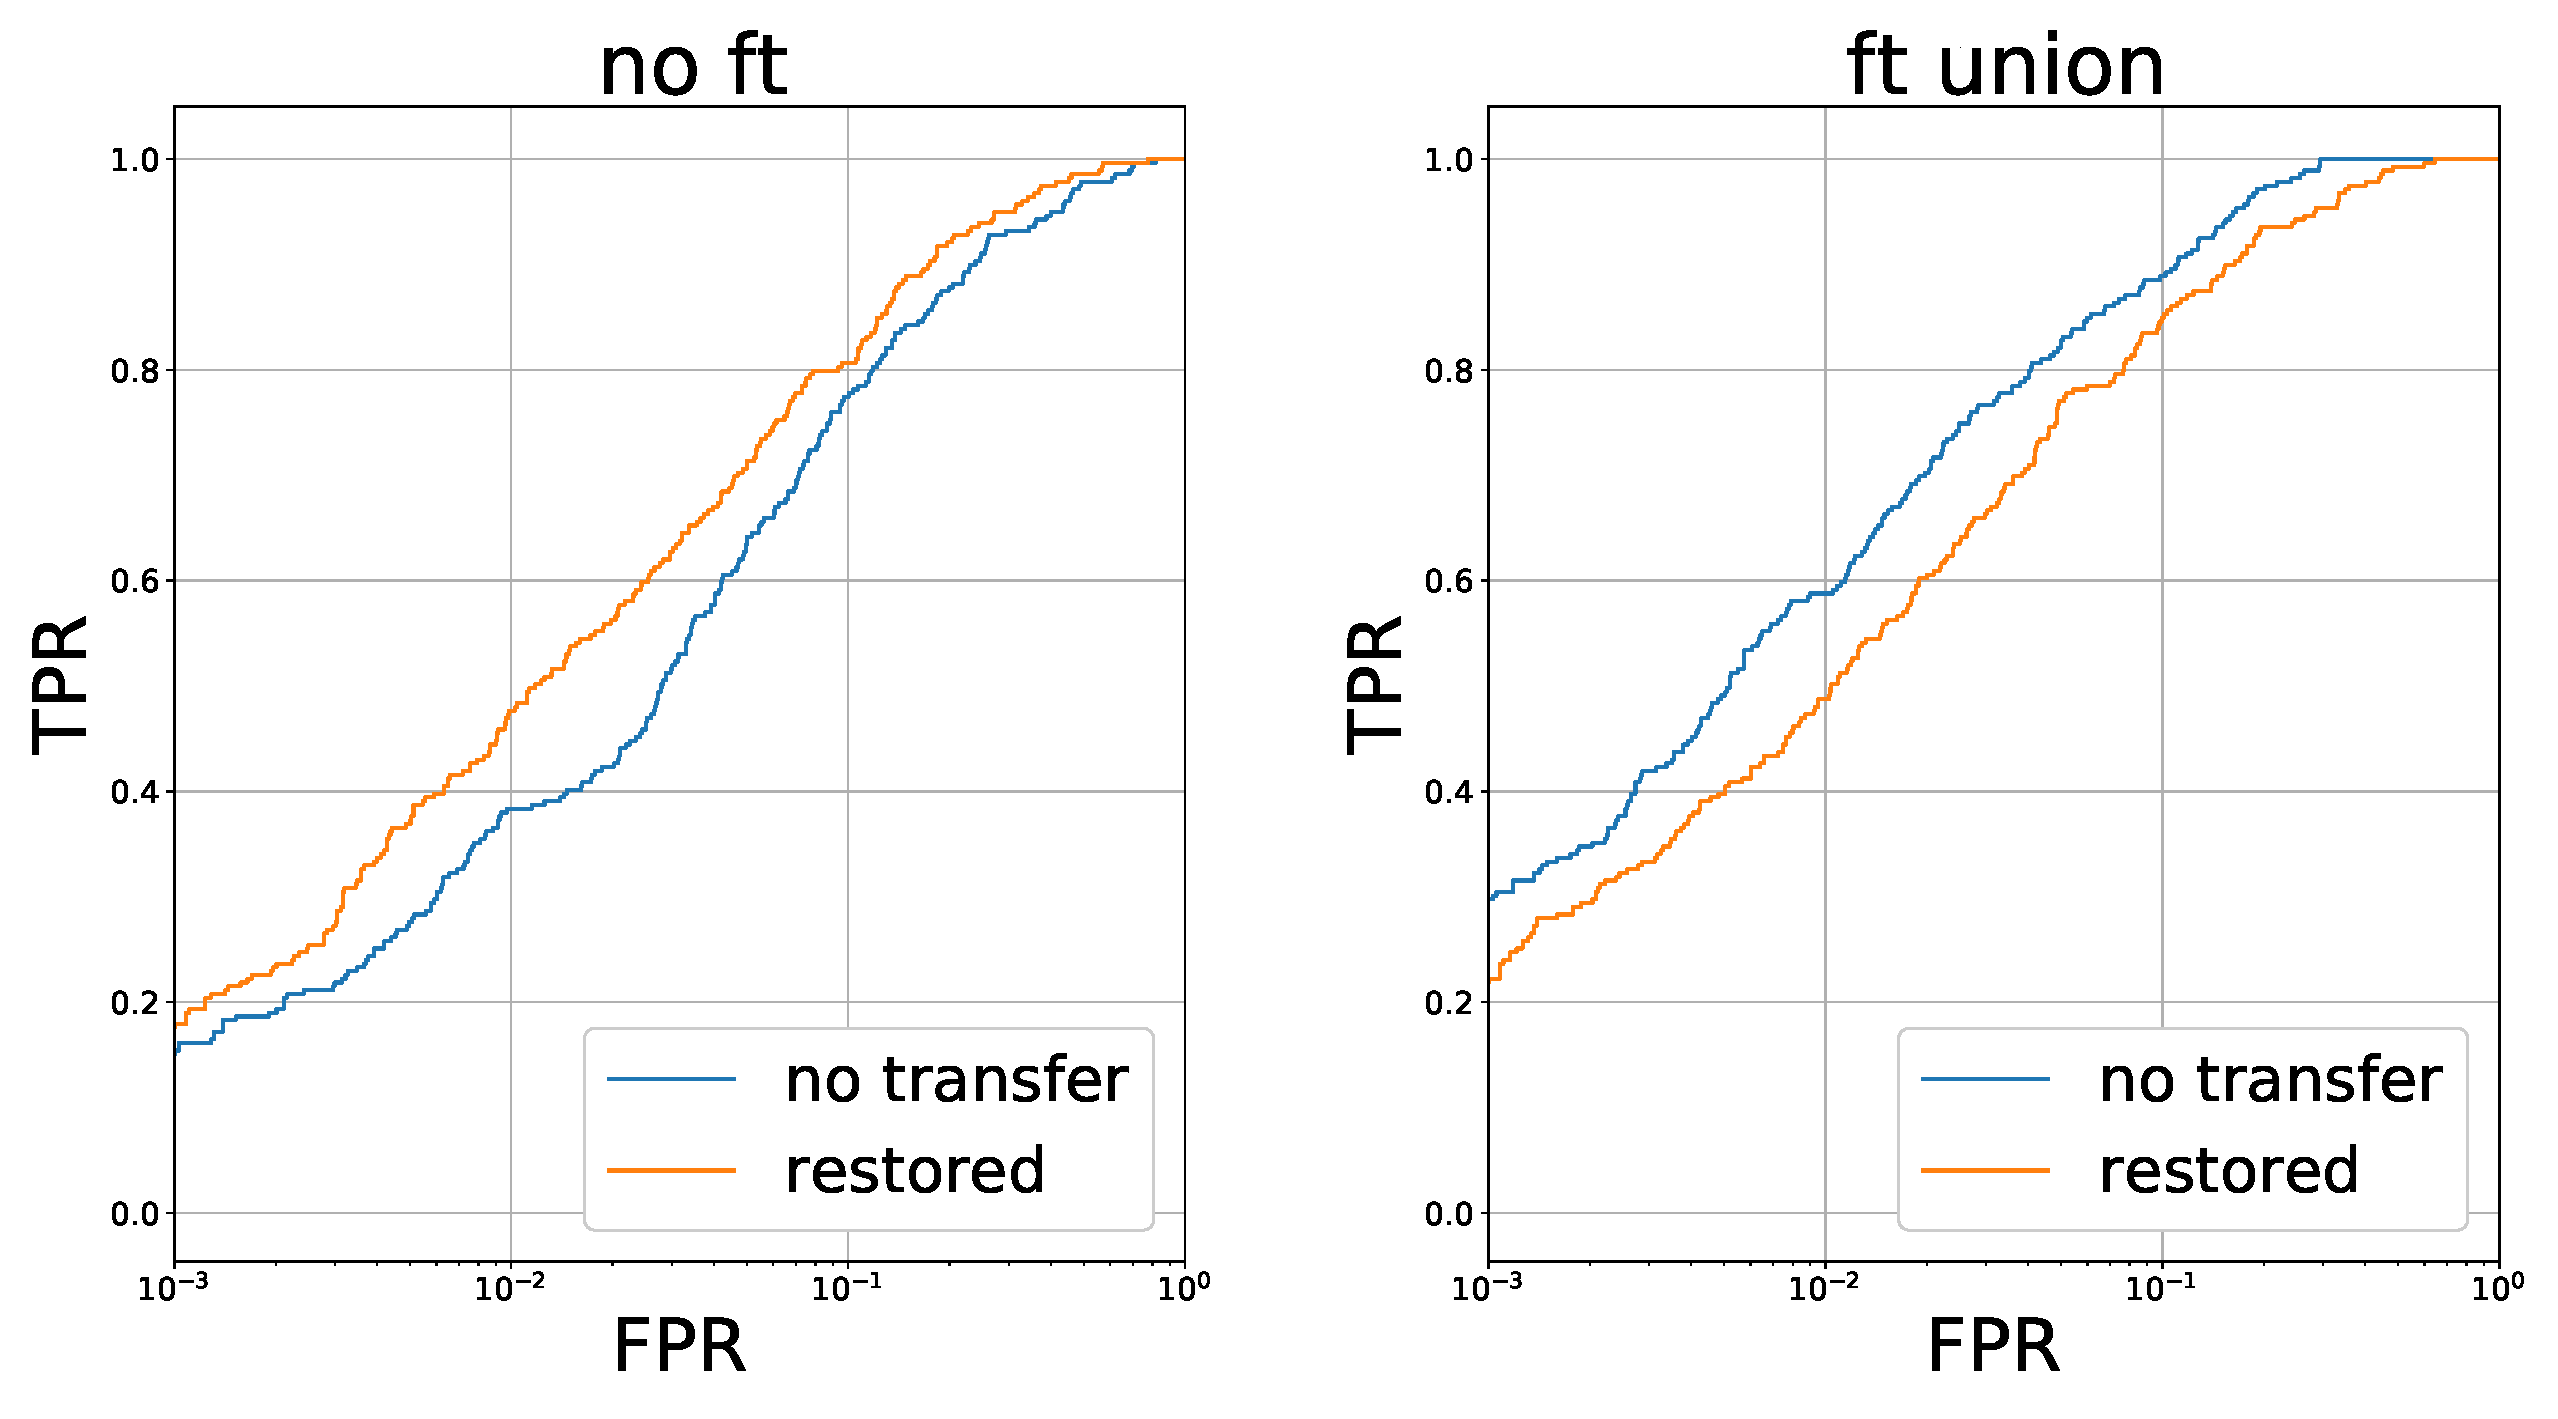
\includegraphics[width=\linewidth]{Chapters/face/Fig4.eps}
    \caption{The change of the recognition metrics for our surveillance validation set. \textit{ft degraded} and \textit{ft union} models that use our image-level domain adaptation overfit less than \textit{ft initial} that use only the initial Internet-domain data. The improvement is consistent across the two cases when VGG face and YTF datasets were used as Internet image data. See subsection \ref{sect:ft} for the models description.}\label{fig:validation_ytube}
  \end{figure}
  
  \begin{figure}

  \centering
    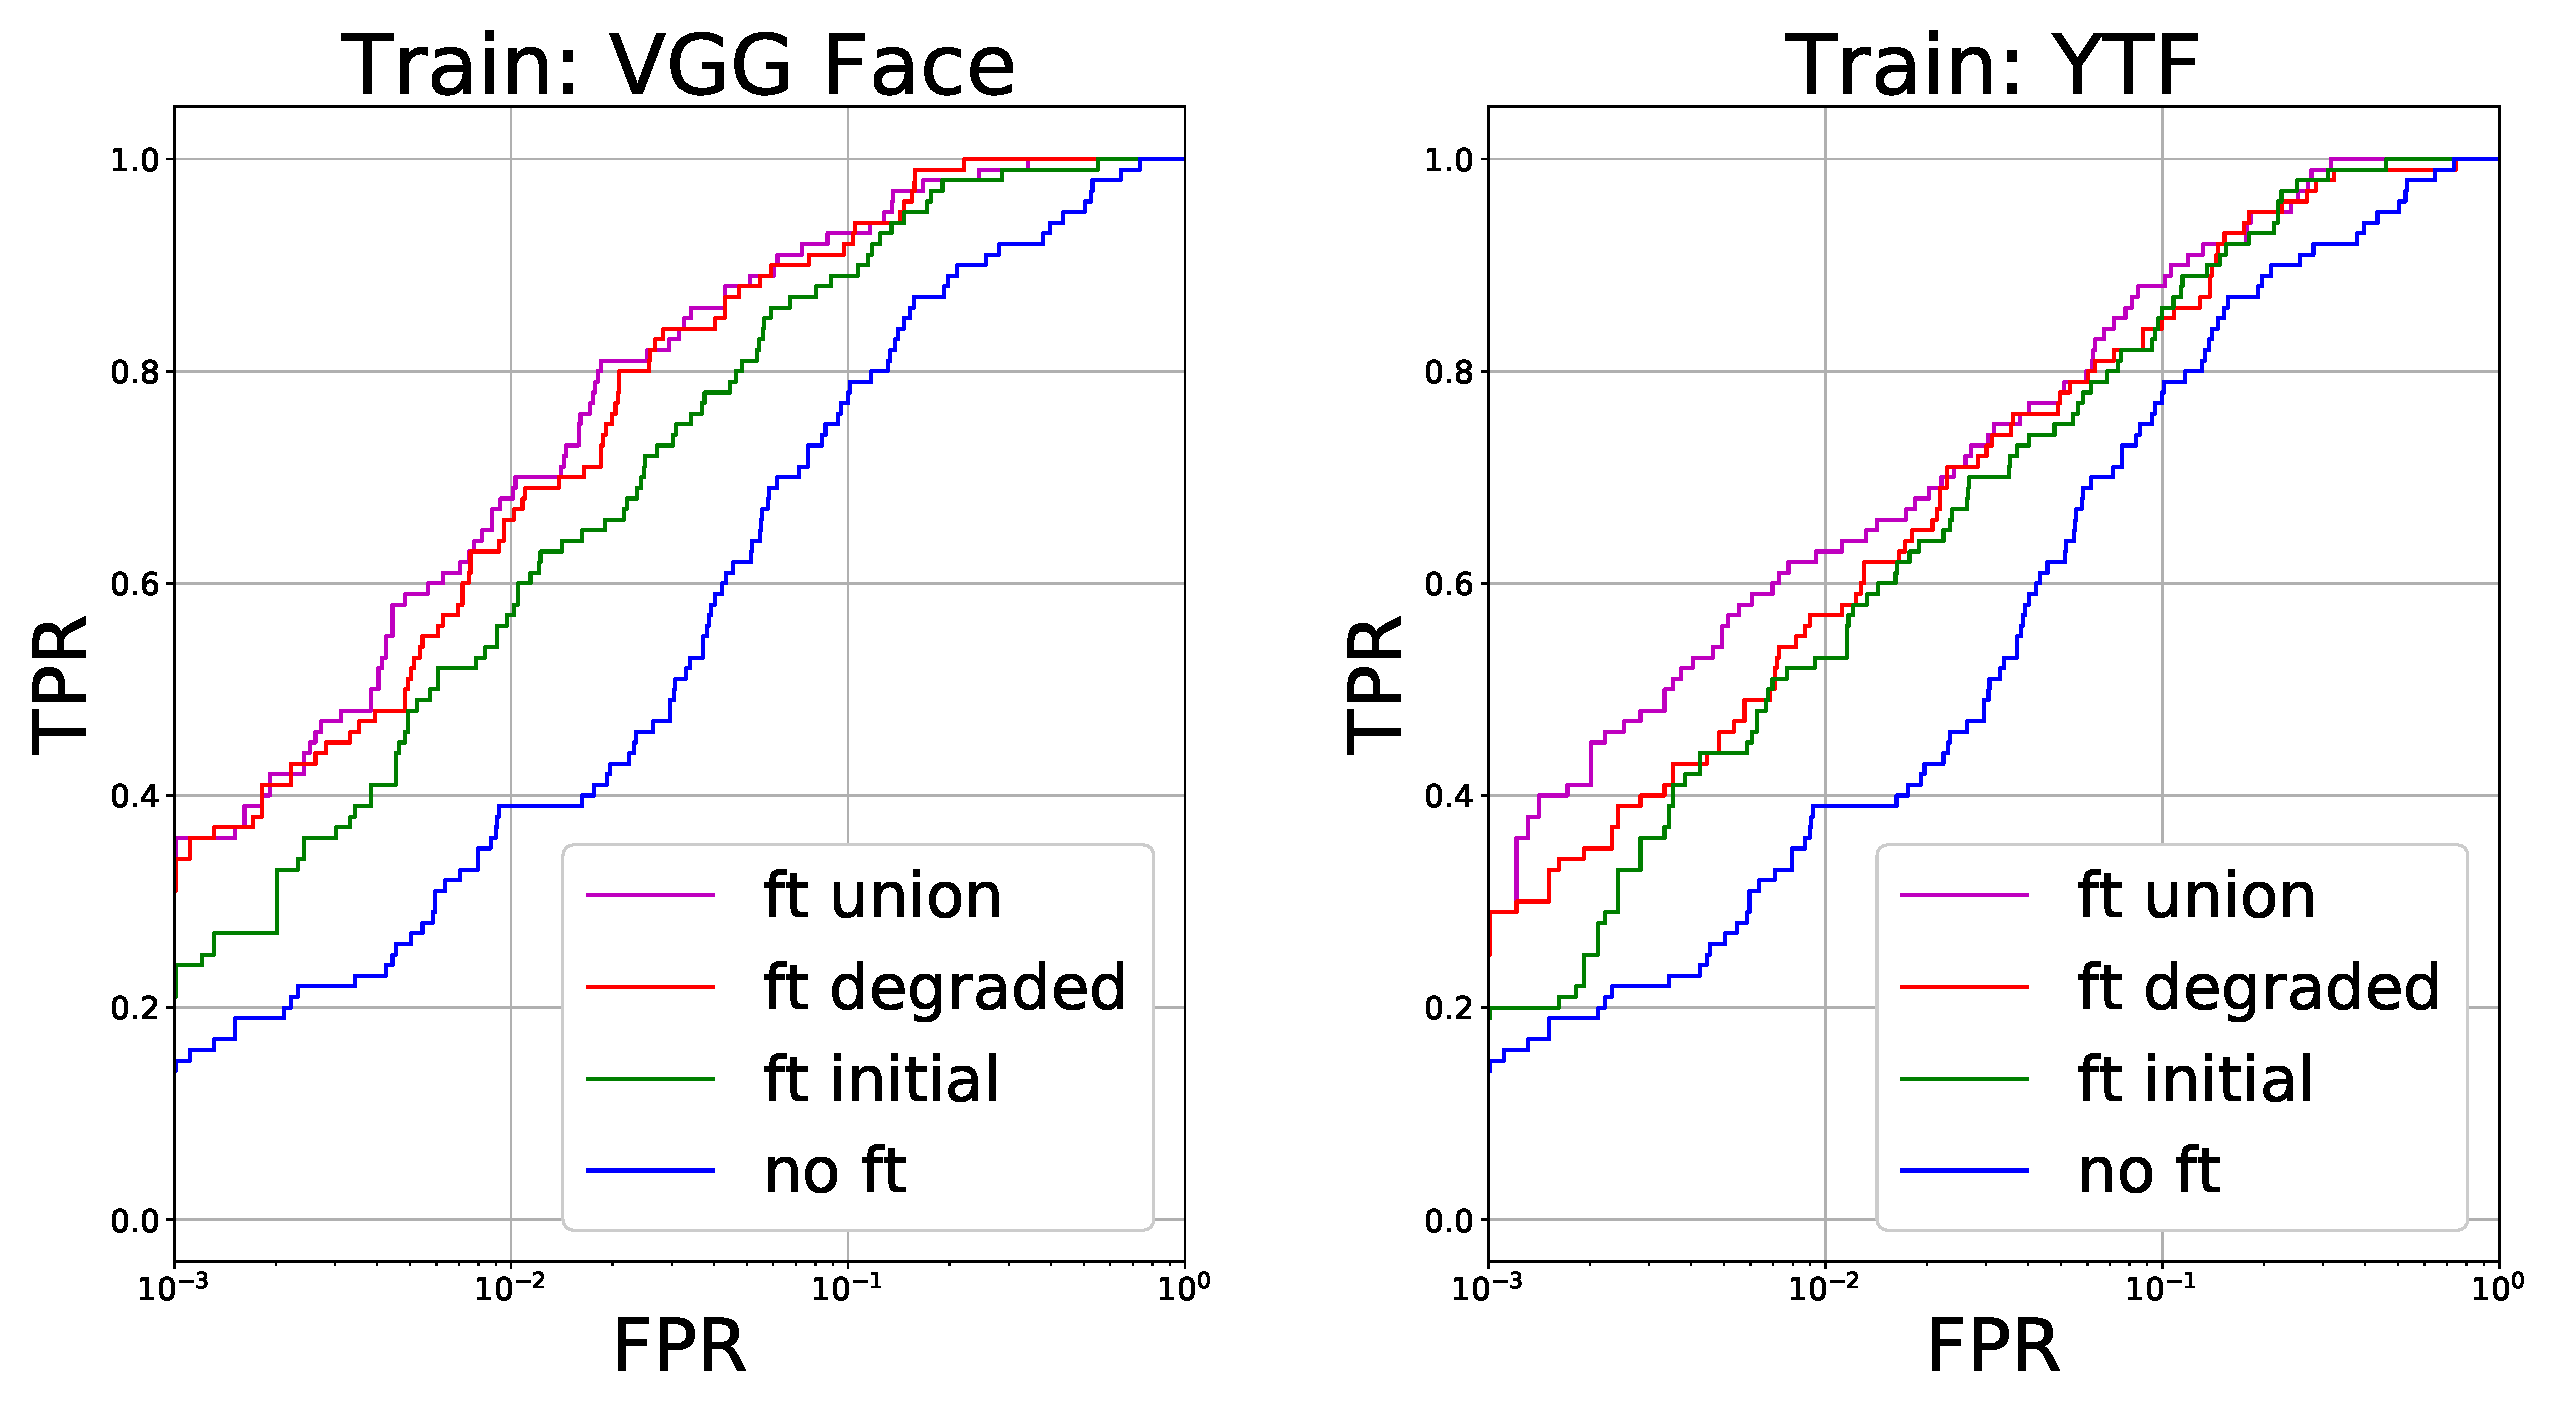
\includegraphics[width=\linewidth]{Chapters/face/Fig5.eps}
    \caption{The ROC curves for the fine-tuning strategies described in \sect{ft}. Our surveillance data is used for test. \textit{ft degraded} and \textit{ft union} models that use our image-level domain adaptation are better than other models. }\label{fig:roc_oxford_ytube}
  \end{figure}
  
 
\begin{table}
\flushbottom

\centering
\caption{Quality metrics for different face recognition models compared in this work (\ref{sect:ft}). The best model is \textit{ft union}, it is trained on both initial and degraded data.}
\label{tab:comparison}
\resizebox{\columnwidth}{!}{
\begin{tabular}{|c|c|c|c|c|c|c|}
\hline
\multicolumn{1}{|l|}{}   & \multicolumn{6}{c|}{Train datasets}                      \\ \hline
\multicolumn{1}{|l|}{}   & \multicolumn{3}{c|}{YTF} & \multicolumn{3}{c|}{VGG Face} \\ \hline
Fine-tuning type & 100\%$-$eer & roc auc & AP & 100\%$-$eer   & roc auc   & AP  \\ \hline
no ft                    &  84.73 & 91.52 & 25.98 &   84.73 & 91.52 & 25.98  \\ \hline
ft initial               &  88.52 & 95.67 & 42.38 &  89.32 & 96.62& 44.10  \\ \hline
ft degraded              &  87.03         & 95.53 &  47.02 & 90.28 &\bf{97.84} &53.33  \\ \hline
ft union                 &  \bf{89.41}    &   \bf{96.45} &\bf{50.91}&    \bf{91.31} &97.80 &\bf{54.89}   \\ \hline
\end{tabular}
}
\end{table}

  
 
%\subsubsection{Does domain adaptation help recognition?}
\bigskip\indent\textbf{Does domain adaptation help recognition?} \\
\label{sect:results}
We now consider the second scenario based on domain adaptation and thus compare the performance of different recognition networks described above on surveillance data. Our findings for image level domain adaptation are summarized in Table~\ref{tab:comparison}, which shows metric values for the compared training settings, and \fig{validation_ytube}, which shows validation metrics changes during training. Finally, \fig{roc_oxford_ytube} shows the final ROC curves.

The following can be observed. First, fine-tuning the VGG Face model on either VGG Face dataset or the YTF dataset using the BinDev loss (\textit{ft initial}) lead to a considerable improvement over the original state of the network.
Furthermore, we found that fine-tuning in the \textit{ft degraded} setting is clearly beneficial compared to \textit{ft initial} setting in the case of the VGG Face training dataset, and a little bit better for the YTF training data, overall making a case for image-level domain adaptation. The results of the \textit{ft union} setting are uniformly better than \textit{ft initial} and \textit{ft degraded} suggesting that the automatically degraded data are a useful augmentation, but that the original data should not be discarded. 
Finally, \fig{tsne} gives an additional evidence of the success of domain adaptation. It shows that the feature distribution of our surveillance data is more intermixed with those of the degraded version of the YTF dataset than its initial version. This demonstrates the relevance of the suggested augmentation (via image-level domain adaptation).



% \subsubsection{Comparison to the reverse domain transfer}
% \label{sect:restoration_comparison}

% We have also investigated the restoration-based approach (\sect{strategies}), using the reverse mapping $F^{S \rightarrow T}$ that also comes out as the result of training the model \ref{sect:domain_transfer}. 
% Here we test our previously trained face recognition models (described in  \sect{ft}) on different variants of test data. See  \fig{lr_hr_gan_res_ytube_initial_degraded} for the example results of the Internet domain  transfer.

% We have evaluated the effect of such reverse transfer to the higher-quality domain at test term for the \textit{no ft}, \textit{ft initial}, and \textit{ft union} networks described in the previous subsection. The ROC-curves in  \fig{roc_oxford_gan_vs_initial} shows that while the reverse transfer helps for the \textit{no ft} network, it actually hurts for the better working \textit{ft initial} and \textit{ft union} networks. While trying to improve the results of the reverse transfer, we have also tried to transfer only the LR subset of the training images, while keeping the HR subset intact, but this lead to uniformly worse results.

%in the case of the pre-trained VGG face network (\textit{no-ft}), transferring low-quality test images into the Internet data domain improves recognition. Nevertheless, if we use one of the fine-tuned models for recognition, the results for the initial test images are not worse than those for transferred images. Moreover, ROC curve for initial test images is the highest for our best \textit{ft union} model as shown in \ref{fig:roc_oxford_gan_vs_initial}-right.



%\subsubsection{Comparison to feature-level domain adaptation}

\bigskip\indent\textbf{Comparison to feature-level domain adaptation} \\
\label{sect:grl}
We have additionally compared our image-level domain adaptation (all the experiments and discussions above) to the feature-level domain-adversarial adaptation approach described in \chapt{gradrev}. Tuning this approach required some effort (several modifications from the settings of \chapt{gradrev} were needed to make such adaptation work). We thus built a DANN (Deep Adversarial Neural Network) based on the VGG-face network. The  domain classifier consists of three fully-connected layers: $512$ units in the first two layers (Leaky ReLU \cite{HeZRS15} non-linearities were used) and one classification layer with $1$ unit. Dropout with $0.5$ probability was inserted before the classification layer. The Gradient Reversal layer is attached after the \textit{fc6} layer of VGG-face. We found that schedule for the adaptation parameter  $\lambda$ is very important for this task. Instead of the schedule suggested in \chapt{gradrev} (which did not lead to good results in our comparison), we set $\lambda$ to $1e-3$ for the first $20$ epochs and then increased it to $1e-2$. 

Using the scheme described above when training on the VGG Face dataset, we have achieved the following results: $100$\% - EER was $88.64$, ROC AUC was $96.69$ and the average precision was $52.11$. This is better than the results of our \textit{ft initial} setting, but worse than those of \textit{ft degraded} and \textit{ft union} settings (for the last, the results are $91.31$, $97.80$ and $54.89$ correspondingly). Other setting for feature-level domain adaptation that we have tried lead to worse results.






  
  
  
  

\subsection{Summary}
\label{sec:summary}
In this work we present a deep neural network for multi-frame face super-resolution that performs alignment, reconstruction and recognition in holistic manner and learns respective modules in the end-to-end fashion. We evaluate different variants of the proposed architecture including single-image baseline. In the experiments on YouTube Faces dataset, we demonstrate the advantages of having the alignment module in the system. In the presence of alignment, we observe the improvement both in visual quality (confirmed by the user study) and in the face recognition accuracy over the single frame baselines and the single frame system \cite{ZhuLLT16}. 

